\clearpage
\section{Mô hình hoá cơ sở - kỹ thuật trong đề cương}
\subsection{Lựa chọn thuật toán}
%Mô hình Hồi quy tuyến tính (Linear Regression) áp dụng trên đặc trưng đơn (ví dụ: GrLivArea). Đây là phần đáp ứng yêu cầu dùng thuật toán trong đề cương môn học.
Trong quá trình xây dựng mô hình cơ sở, nhóm lựa chọn \textbf{Hồi quy tuyến tính đơn giản (Simple Linear Regression)}. Đây là một thuật toán nền tảng trong học máy, thường được sử dụng để thiết lập baseline trước khi thử nghiệm các mô hình phức tạp hơn. \medskip

Nhóm sẽ sử dụng Heatmap tương quan để quan sát sự tương quan giữa các thành phần với SalePrice.
\begin{figure}[H]
    \centering
    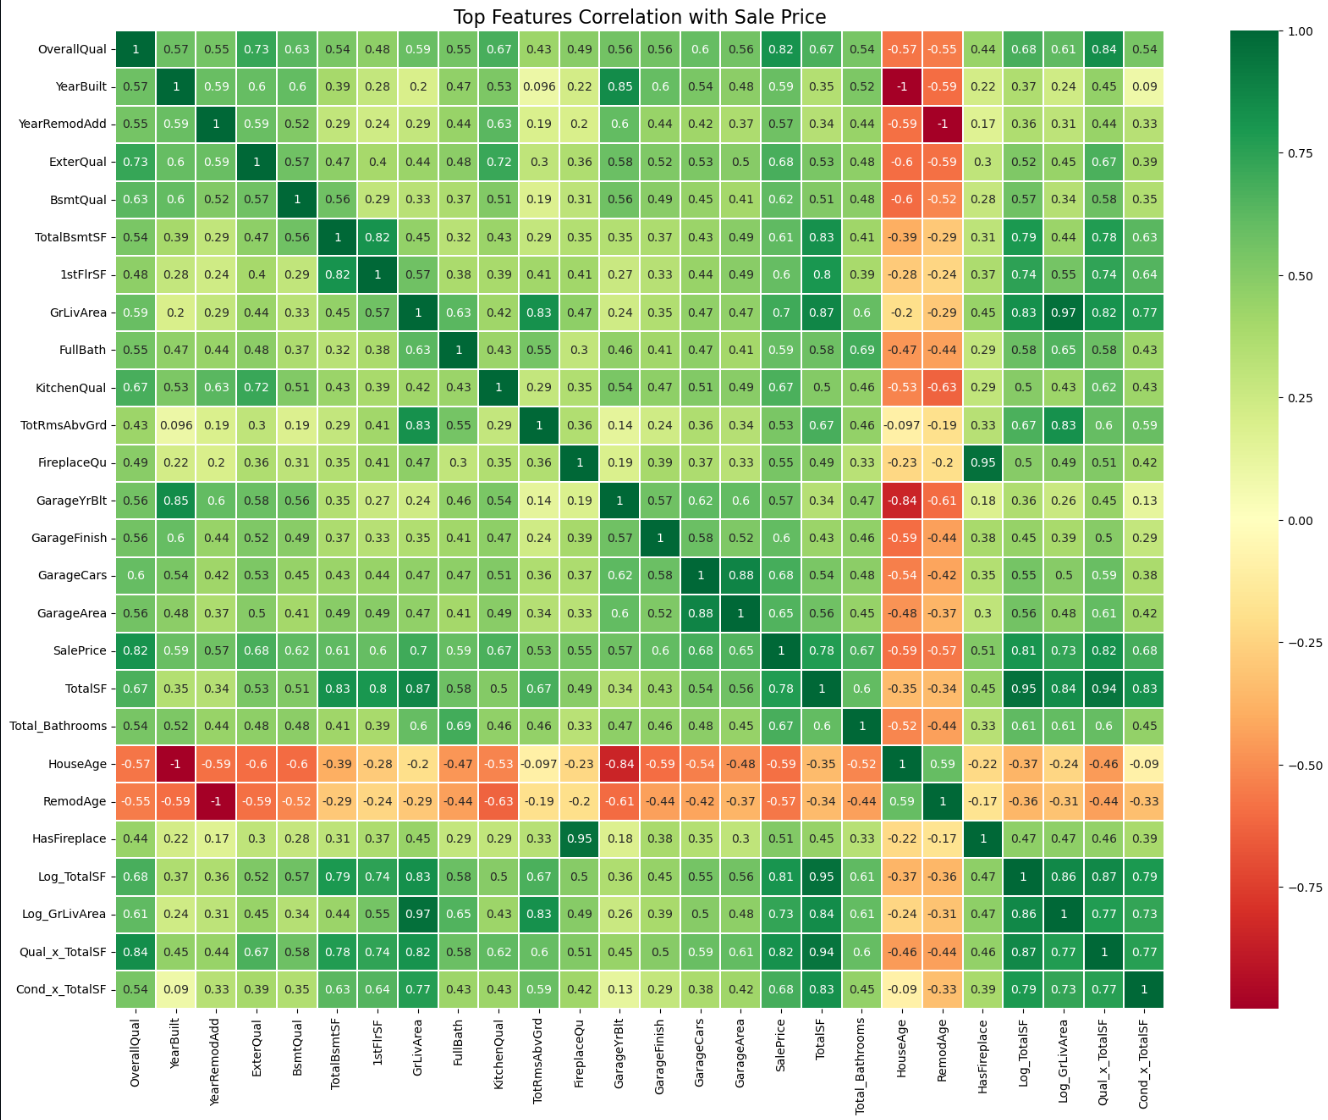
\includegraphics[width=1\linewidth]{images/baseline_model/Heatmap.png}
    \caption{Heatmap tương quan giữa các thành phần với SalePrice}
\end{figure}
Sau khi quan sát biểu đồ Heatmap thì một số biến có độ tương quan với SalePrice vượt ngưỡng 0.7 là: Qual\_x\_TotalSF (0,82), Log\_GrLivArea (0.73), Log\_TotalSF (0.81), TotalSF (0.78), GrLivArea (0.7), OverallQual (0.82).
\subsubsection{Cơ sở lựa chọn:}
\begin{itemize}
    \item[-] Qua phân tích biểu đồ tương quan, nhiều biến có hệ số tương quan cao với SalePrice như OverallQual, TotalSF, Log\_TotalSF. Tuy nhiên, các biến này phần lớn là kết quả của quá trình tiền xử lý hoặc kết hợp nhiều đặc trưng. Để đảm bảo tính đơn giản, trực quan và dễ diễn giải, nhóm đã lựa chọn GrLivArea - một đặc trưng gốc phản ánh diện tích sinh hoạt
    \item[-] Nhóm sau đó sử dụng thêm biểu đồ phân tán (scatter plot) giữa GrLivArea và SalePrice để minh họa xu hướng tuyến tính rõ rệt: khi diện tích sinh hoạt càng lớn thì giá bán nhà càng cao.
\end{itemize}
\begin{figure}[H]
    \centering
    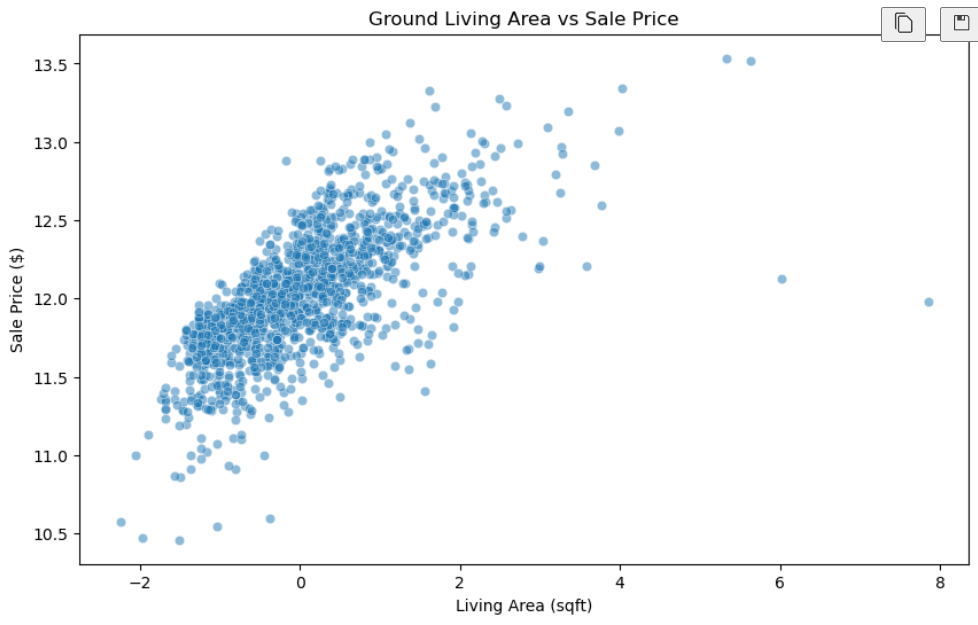
\includegraphics[width=1\linewidth]{images/baseline_model/Scatter.png}
    \caption{Tuyến tính giữa GrLivArea và SalePrice}
\end{figure}
\begin{itemize}
    \item[-] Do mối quan hệ tuyến tính nổi bật, nhóm lựa chọn \textbf{Hồi quy tuyến tính đơn giản (Simple Linear Regression)} làm mô hình cơ sở.
    \item[-] Đây là thuật toán nền tảng, dễ triển khai và dễ diễn giải, phù hợp để thiết lập baseline trước khi thử nghiệm các mô hình phức tạp hơn.
\end{itemize}
\subsubsection{Ý nghĩa của việc chọn mô hình cơ sở:}
\begin{itemize}
    \item[-] Thiết lập chuẩn mực ban đầu để so sánh hiệu quả cải thiện khi áp dụng các mô hình đa biến hoặc phi tuyến tính.
    \item[-] Kiểm chứng giả thuyết rằng diện tích sinh hoạt là một yếu tố quan trọng trong việc định giá nhà.
    \item[-] Cho phép trực quan hóa mối quan hệ giữa biến đầu vào và biến mục tiêu, từ đó phát hiện những giới hạn của mô hình này. 
\end{itemize}
\subsection{Huấn luyện và Đánh giá}
%Phân tích các chỉ số đánh giá (RMSE, R-squared) và đồ thị phân dư (Residuals).
\subsubsection{Quá trình huấn luyện:}
\begin{itemize}
    \item[-] Dataset sẽ được chia thành Training set (80\%) và Validation set (20\%).
\end{itemize}
\begin{figure}[H]
    \centering
    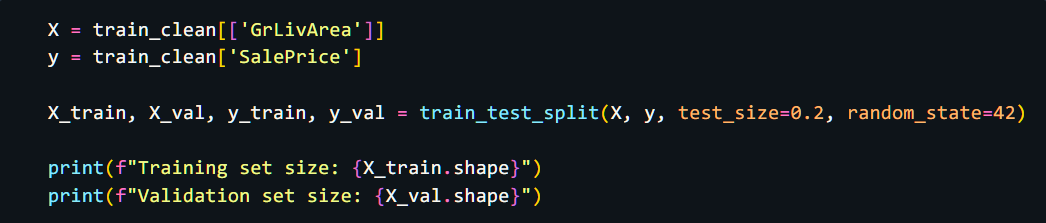
\includegraphics[width=0.8\linewidth]{images/baseline_model/SplitDataset.png}
    \caption{Chia Dataset thành Training và Validation set}
\end{figure}
\begin{itemize}
    \item[-] Sau khi thực hiện chia dữ liệu thành các tập training và validation thì nhóm đưa dữ liệu vào mô hình để huấn luyện.
\end{itemize}
\begin{figure}[H]
    \centering
    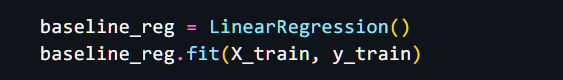
\includegraphics[width=0.5\linewidth]{images/baseline_model/Model.png}
    \caption{Đưa dữ liệu vào mô hình}
\end{figure}
\begin{itemize}
    \item[-] Sau khi huấn luyện, mô hình được dùng để dự đoán giá nhà trên tập dữ liệu kiểm định.
\end{itemize}
\subsubsection{Trực quan hóa kết quả mô hình:}
\begin{itemize}
    \item[-] Để kiểm chứng hiệu quả của mô hình hồi quy tuyến tính đơn giản, nhóm biểu diễn đường hồi quy (regression line) trên tập kiểm định và phân tích sai số qua biểu đồ sai số (residual plot).
\end{itemize}
\begin{figure}[H]
    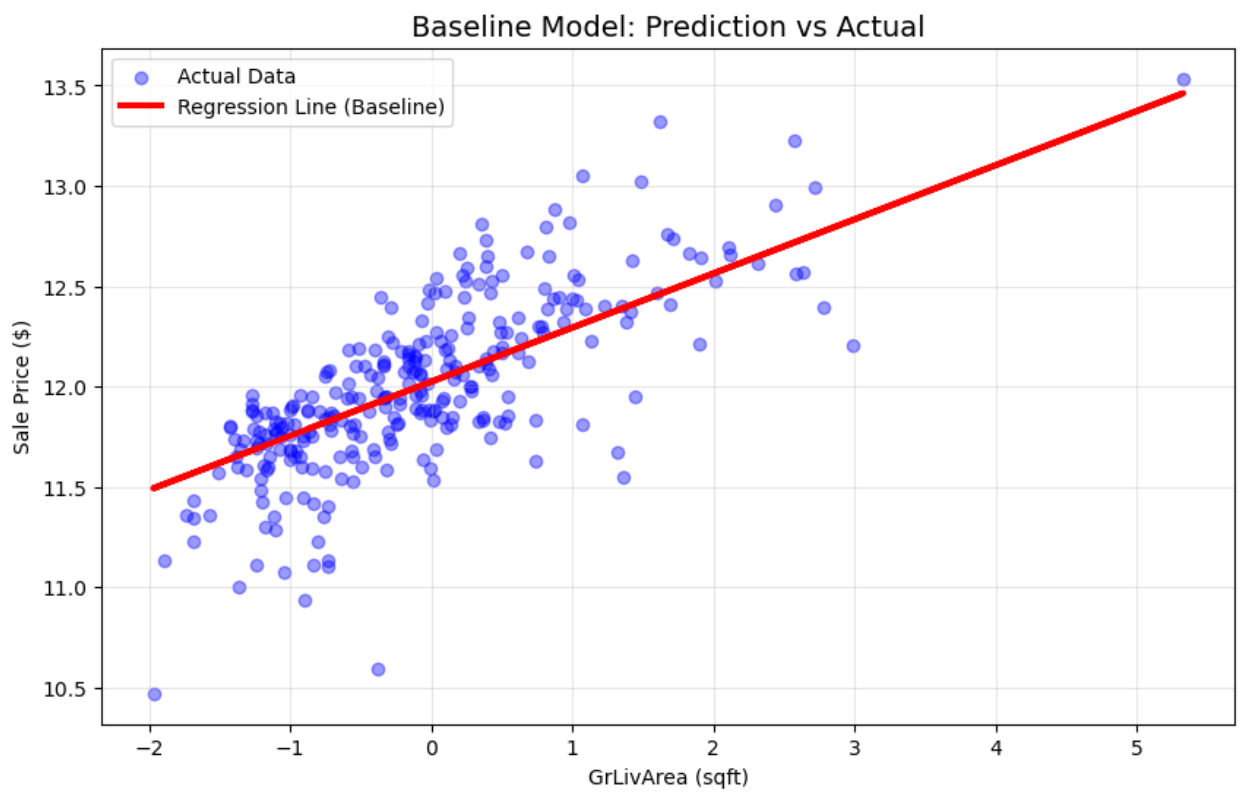
\includegraphics[width=1\linewidth]{images/baseline_model/RegressionLine.png}
    \caption{Đường hồi quy tuyến tính giữa GrLivArea và SalePrice trên tập kiểm định}
\end{figure}
\begin{figure}[H]
    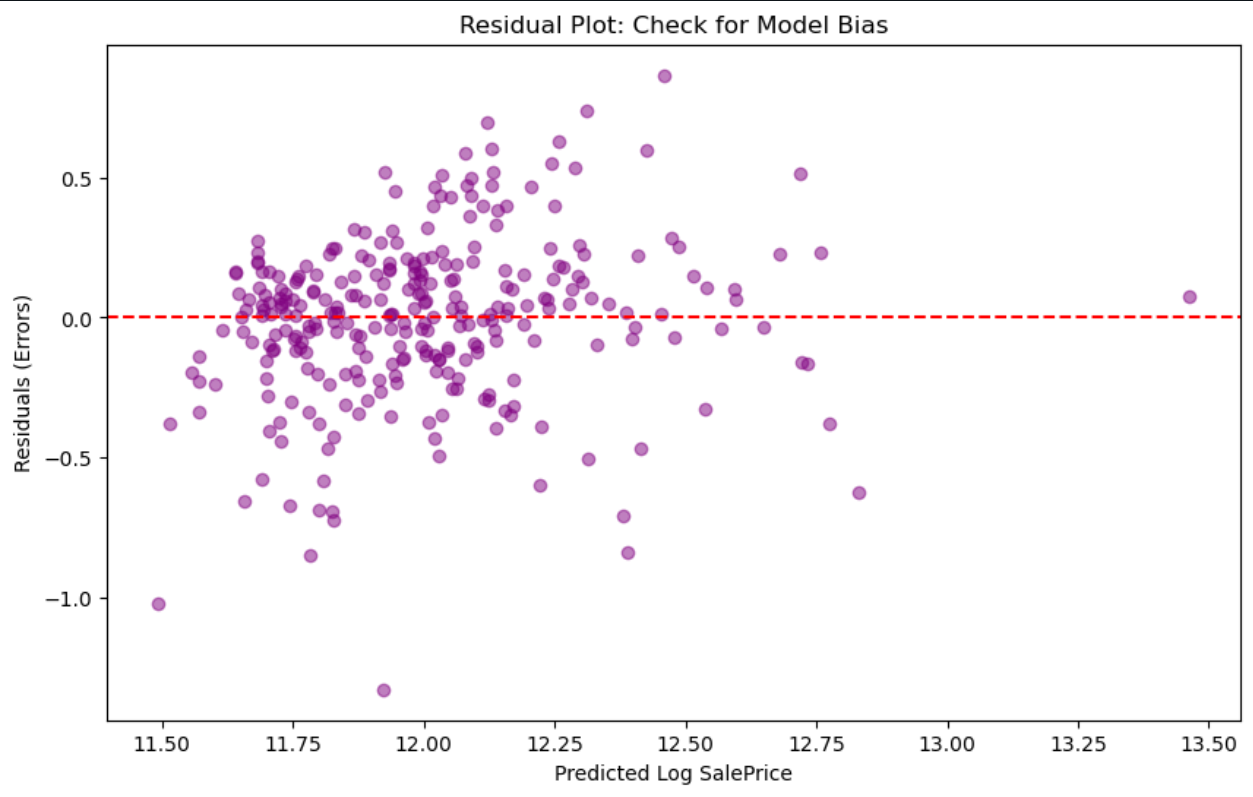
\includegraphics[width=1\linewidth]{images/baseline_model/ResidualPlot.png}
    \caption{Biểu đồ sai số (Residual Plot) kiểm tra độ lệch của mô hình}
\end{figure}
\subsubsection{Kết quả đánh giá:}
\begin{itemize}
    \item[-] Nhóm sẽ sử dụng công thức RMSE (Root Mean Squared Error) để đo lường độ lệch trung bình giữa giá trị dự đoán và giá trị thực tế và công thức R-squared để nhận biết mô hình giải thích được bao nhiêu phần trăm biến thiên của dữ liệu.
    \item[-] Công thức RMSE: 
\begin{equation}
RMSE = \sqrt{\frac{1}{n} \sum_{i=1}^{n} (y_i - \hat{y}_i)^2}
\end{equation}
    \item[-] Công thức R-Squared: 
\begin{equation}
R^2 = 1 - \frac{SS_{res}}{SS_{tot}} = 1 - \frac{\sum_{i=1}^{n} (y_i - \hat{y}_i)^2}{\sum_{i=1}^{n} (y_i - \bar{y})^2}
\end{equation}
    \item[-] RMSE (Root Mean Squared Error): \$58,137.54 
    \item[-] R-Squared: 0.5402
\end{itemize}
\subsubsection{Diễn giải kết quả:}
\begin{itemize}
    \item[-] Mô hình giải thích được khoảng 54\% sự biến thiên của giá nhà, xác nhận rằng diện tích sinh hoạt là một biến dự báo mạnh.
    \item[-] Tuy nhiên, sai số trung bình khoảng \$58k là khá lớn, cho thấy mô hình bỏ qua nhiều yếu tố quan trọng khác.
    \item[-] Biểu đồ residual cho thấy sai số phân tán rộng, chứng minh rằng mô hình tuyến tính đơn biến chưa đủ để mô tả toàn bộ dữ liệu. 
\end{itemize}

\subsection{Nhận xét giới hạn của mô hình cơ sở}
\subsubsection{Những giới hạn chính:}
\begin{enumerate}
    \item Đơn biến:
    \begin{itemize}
        \item[-] Mô hình chỉ sử dụng một đặc trưng duy nhất (GrLivArea).
        \item[-] Bỏ qua các yếu tố quan trọng khác như chất lượng xây dựng (OverallQual), tổng diện tích (TotalSF), vị trí địa lý, tuổi thọ căn nhà, số phòng, ...
    \end{itemize}
    \item Giả định tuyến tính:
    \begin{itemize}
        \item[-] Hồi quy tuyến tính đơn giản giả định mối quan hệ tuyến tính hoàn toàn giữa diện tích sinh hoạt và giá nhà.
        \item[-] Thực tế, giá nhà thường chịu ảnh hưởng phi tuyến tính và tương tác giữa nhiều biến. 
    \end{itemize}
    \item Sai số cao:
    \begin{itemize}
        \item[-] RMSE ~ \$58k là mức sai số lớn, không đủ để ứng dụng trong thực tế.
        \item[-] Biểu đồ residual cho thấy sai số phân tán rộng, chứng minh mô hình chưa nắm bắt hết cấu trúc dữ liệu.
    \end{itemize}
    \item Khả năng khái quát hạn chế:
    \begin{itemize}
        \item[-] Mô hình cơ sở chỉ phù hợp để minh họa xu hướng tổng quát, không thể dự đoán chính xác cho từng trường hợp cụ thể.
    \end{itemize}
\end{enumerate}
\subsubsection{Chiến lược cải thiện:}
\begin{itemize}
    \item[-] \textbf{Hồi quy đa biến:} Kết hợp nhiều đặc trưng có tương quan cao với SalePrice.
    \item[-] \textbf{Thuật toán phi tuyến tính:} Áp dụng Random Forest, Gradient Boosting hoặc XGBoost để nắm bắt quan hệ phức tạp.
    \item[-] \textbf{Feature engineering:} Sử dụng các biến đã qua xử lý (log-transform, kết hợp đặc trưng) để giảm sai số.
\end{itemize}